\documentclass[12pt]{article}
\usepackage[utf8]{inputenc}
\usepackage{amsmath}
\usepackage{amsfonts}
\usepackage{amssymb}

\usepackage[margin=1in]{geometry} %1inch margins
\usepackage{graphicx} %for picture inclusion
\graphicspath{ {Figures/} }
\usepackage[backend=bibtex]{biblatex} %for references
\addbibresource{ref.bib} % bibliography info file
\usepackage{authblk} %for titles
\usepackage{verbatim}

\begin{document}

\author{Daniel Gawerc\\Mentor: Maria Spiropulu\\Co-Mentor: Cristian Peña}
\affil{California Institute of Technology}
\title{Progress Report \#2}
\date{29 July 2016}
\maketitle

\section{Background}
At the Large Hadron Collider (LHC), the High Luminosity upgrades plan to achieve luminosities of greater than $10^{34}$ cm$^{-2}$s$^{-1}$, with 140 – 200 pileup events per bunch crossing every 25 ns \cite{P1}. 
Because of the physical spread of each bunch, the collisions occur over a large region rather than at an isolated point, which leads to a spread in time ($\sim$ 200 ps) \cite{P1}. 
Thus, detectors in the calorimeter must have a good (low) time resolution in order to resolve individual collisions. 
In order to reconstruct the vertex of a collision with an increased pileup, the electromagnetic calorimeter (ECAL) detectors should have a time resolution of about 10 ps \cite{P1}.


\section{Experimental Setup}
This summer, the Caltech Precision Timing group took data at the Fermilab Test Beam Facility (FBTF). 
The experiment involves placing different calorimeter detectors in the beam line, in order to observe how the addition of detectors in the perpendicular transverse plane and/or parallel longitudinal direction along the beam line will improve the overall detector time resolution. 
The layers of detectors are meant to mimic the proposed High Granularity Calorimeter (HGC) detector, which shall replace the CMS ECAL endcap, and is described in detail below \cite{P2}. 
The results of this research may be useful in preparing the LHC High Luminosity upgrades.

In the FTBF experiment, different types of detectors were utilized. 
In the front of the setup, a scintillator crystal and PMT are used as a trigger. 
Depending on the configuration, there are a few radiation lengths ($X_0$) of either lead or tungsten absorbers behind the PMT in order to spread out and propagate the particle shower and produce more secondary electrons and photons. 
A depiction of the setup is given in Figure \ref{fig:setup}.

\begin{figure}
	\centering
	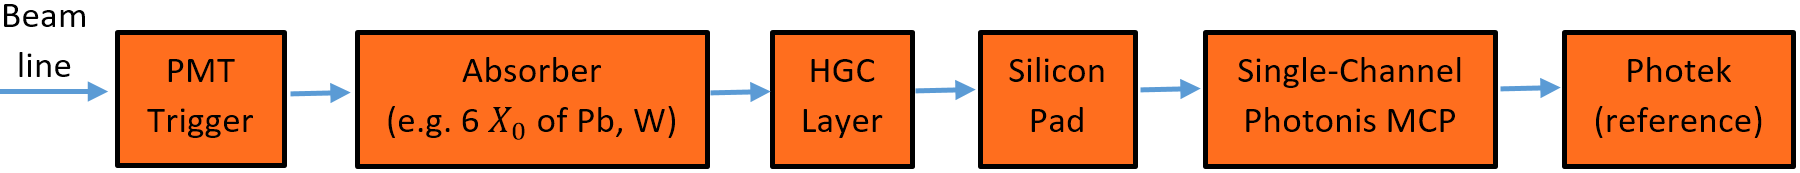
\includegraphics[width=\linewidth]{setup.png}
	\caption{A typical experiment configuration.}
	\label{fig:setup}
\end{figure}

The High Granularity Calorimeter (or PicoSil when referring to a single pixel’s readout that has been optimized for timing) layer has an array of separated silicon pixels, in a hexagonal honeycomb geometry \cite{P2}. 
A depiction of the HGC layer is given in Figure \ref{fig:HGC}. 
Because the beam is focused at the HGC center pixel (0 in Figure \ref{fig:HGC}), its signal is reduced using a 6 dB attenuator due to the high charge detected relative to other pixels. 

The Photek 240 MCP is used as a reference detector because its time resolution is good ($\sim$ 10 ps). 
Because the readout board for all the detectors is divided into 4 groups, which have some time delay between them, the Photek signal is split into 4 cables and plugged into each group as the reference signal from which the TOFs (time of flight, or $\Delta t$) are calculated. 
Specifically, the time taken for the particle to travel from a device to the reference Photek - the time of flight – is represented by $\Delta t$. 
In the data analysis, the $\Delta t$ values over all events in the run (with certain \textit{bad} events excluded) are combined in a histogram, forming a Gaussian peak. 
The peak $\sigma$ parameter is denoted the time resolution.

\begin{figure}
\centering
\begin{minipage}{.5\textwidth}
	\centering
	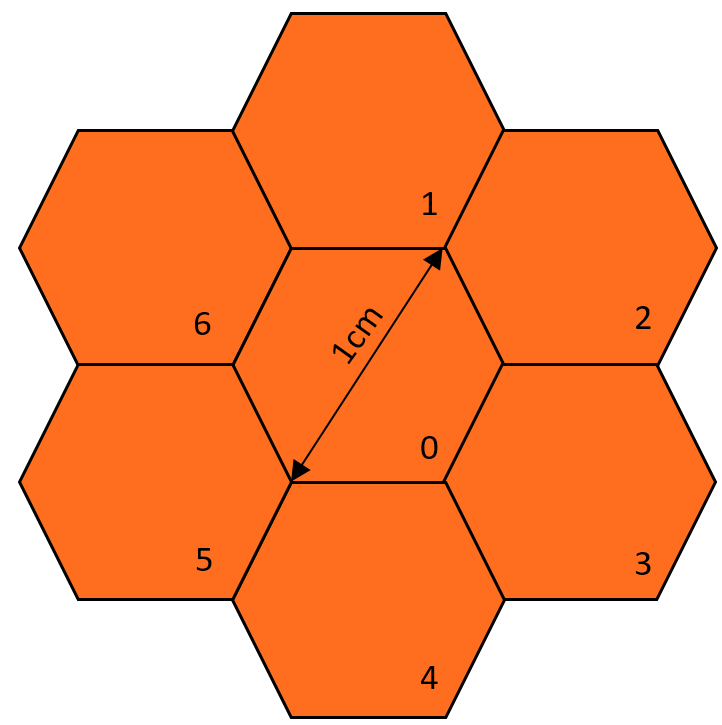
\includegraphics[scale=0.5]{HGC.png}
	\caption{A depiction of the innermost 7 pixels of the HGC layer. 
	The actual board has more than 7 pixels in a single layer.}
	\label{fig:HGC}
\end{minipage}
\end{figure}

There is a 64-channel and a single-channel Photonis MCP. 
The 64-channel Photonis was not present for most runs, and the single-channel Photonis was instead used. 
Lastly, a silicon pad (SiPad) detector was present for most runs, however it only detected pulses well in the very early runs, and does not seem to be useful in most of the analysis.

\section*{3.1 Data Analysis: Overview}
The Caltech Precision Timing group already had developed some analysis code for previous test beam experiments. 
The program \textit{dat2rootCP} analyzes the .dat files (with low-level information) from the runs and turn them into .root files containing a tree with plots and fit results (higher-level information). 
Since some of the data contained ringing noise, which often resulted in the wrong peak being identified as the pulse, \textit{dat2rootCP} was updated to correct for these events. 
Additionally, new macros were written in order to automate batch file analyses and merging the results into a single .root file (for when the setup configuration and beam type were the same over many runs). 
These programs utilize the ROOT programming language, which is based largely on C++. 
It is the main programming language used by scientists at CERN and in the field of HEP (see: root.cern.ch).  
The .root file extensions are associated with the ROOT language.

Because the HGC layer has multiple pixels, each pixel detects different signals and has a different time resolution. 
The \textit{MultiChannelStudy} code was created (here channel and pixel are used interchangeably), which calculates and combines the TOF ($\Delta t$) histograms for different pixels in order to return a better overall time resolution. 
The $\Delta t$ values are calculated for every event in a run by subtracting the pulse time in one device from the pulse time in the Photek (making sure that it is from the same cabling group 1-4 as the device). 
A 1-D histogram is then filled event-by-event with the $\Delta t$ values. 
In an ideal world with perfect detectors and no variation in each event, the histogram would be a Dirac delta function with a time resolution of zero. 
However, due to detector jitter, the signal-to-noise ratio and the particle shower development in the material will vary event-by-event, resulting in Gaussian histograms \cite{P2}. 
After fitting the histogram to a Gaussian, the $\sigma$ parameter gives the time resolution of the detector/pixel. 
If weighted correctly, combining the HGC pixels’ $\Delta t$ histograms will result in a combined histogram with better time resolution (smaller $sigma$). 
This improvement is due to the combination of non-overlapping information about the shower size and development in each of the detectors.

Because there are also multiple devices along the beam line as well as multiple HGC pixels, the analysis of the coplanar HGC pixels has been called \textit{transverse analysis}, and the analysis of multiple devices \textit{longitudinal analysis}. 
This report shall deal mainly with the longitudinal analysis, analyzing the improvement in the time resolution when taking the HGC layer, single-channel Photonis MCP, and SiPad into account. 
However since it is best to use the time resolution from the entire HGC layer, much of the transverse analysis will be done as well. 
Due to re-cabling the wires of the detectors into different groups between runs 52 and 53, I wrote a longitudinal analysis code for the initial setup (with the initial array values) and then another code for the revised setup (the only difference in the codes being which array elements I called). 
Additionally, the SiPad has very prominent noise for all of the runs I have analyzed so far and actually substantially deteriorates the combined detector time resolution. 
For example, Figures 1 and 2 give the time of flight ($\Delta t$) histograms for runs 65-83 (same configuration) for the PicoSil center pixel and the MCP, along with their Gaussian fit $\sigma$ parameter. 
Figure 3 gives the same but for the SiPad. 
Figure 4 is one of the possible combination histograms (depending on how the individual $\Delta t$ histograms are combined; more about this later). 
Clearly the combined histogram improves the SiPad resolution by about 4 times, but it is 3-4 times \textit{worse} than the individual resolutions of the PicoSil and MCP. 
Additionally, the SiPad histogram is peaked, but certainly not Gaussian. 
Note: The PicoSil distribution is also clearly not perfectly Gaussian because it has a tail on the right side, but it is approximately Gaussian (there was maybe an issue with the run, the electronics, or the imposed cut), and the fit $\sigma$ takes it into account. 
Thus, because it is usually more favorable to simply exclude the SiPad, I also created variations of the code that does not account for the SiPad.

%%% INSERT FOUR FIGURES HERE %%%

Therefore, because of the change in cabling and the noise in the SiPad, I created for longitudinal analysis codes: \textit{MultiDeviceStudy}, \textit{MultiDeviceStudy\_InitialWiring}, \textit{MultiDeviceStudy\_PicosilMCP}, and \textit{MultiDeviceStudy\_InitialWiring\_PicosilMCP}. 
Because the most applicable file is \textit{MultiDeviceStudy\_PicosilMCP}, I have made it more extensive than the other three by incorporating all of the ring 1 pixels (the 6 pixels surrounding the center pixel) in the analysis. 
Thus, the code I wrote implements both the transverse analysis of the PicoSil as well as the longitudinal analysis by adding the MCP.

\section*{3.2 Data Analysis: Event Selection}
Before I elaborate upon the different ways to combine the $\Delta t$ of all the pixels of the PicoSil with the MCP, I should explain the cuts that I implement in order to generate the individual $\Delta t$ histograms. 
Because not every event contains a detected pulse, and some have a lot of ringing noise and a negligible pulse, some events need to be cut out of the $\Delta t$ calculations. 
In order to ensure that most of the “bad” events are removed from the histograms, I cut on the calculated peak amplitude and overall charge of the event in that detector, forcing them both to be higher than some threshold. 
This requires that the peak found is not just noise and that the charge (found by integrating the plot) is significant enough to represent a peak.

For example, analyzing the data (with \textit{dat2rootCP}) from run 65 returns a maximum amplitude value in the Photek for every event. 
Filling a histogram with all of these values in the command-line in ROOT gives Figure 1. 
Clearly the amplitudes that are near zero or negative are events without pulses or very noise events. 
These events should be ignored, so a cut shall be implemented to only select for events with the amplitude above a certain value. 
In this case the value appears to be about 0.1. 
Figure 2 shows the histogram of the amplitudes with only the events that passed the cut.

%%% INCLUDE 2 FIGURES %%%

Similar cuts were made for the amplitude and charge in the Photek, PicoSil pixels, and Photonis MCP. 

\section*{3.3 Data Analysis: Device Combination}
The \textit{MultiDeviceStudy\_PicosilMCP} code currently outputs 12 $\Delta t$ histograms. 
The simplest are the PicoSil center pixel and the single-channel Photonis MCP histograms (Figures 1 and 2). 
Another histogram (Figure 3) is the average value of the center pixel and the MCP $\Delta t$ at every event. 
Figure 4 adds in the other 6 pixels of the inner ring of the PicoSil, and weights everything by taking the arithmetic average of the $\Delta t$’s for the devices that passed the cuts.

	Another histogram (Figure 5) averages all 7 of the PicoSil $\Delta t$’s equally, and then averages that value with the MCP:

\[
\Delta t_i = \dfrac{ \Delta t_{MCP_i} }{2} + \dfrac{\sum \Delta t_{PicoSil_i} }{14}
\]

However, the last two combinations (Figures 4/5) are not the best ways to combine the pixels in the PicoSil. 
Due to the electromagnetic nature of the particle beam, the shower spreads out as it evolves, so more particles will pass through some of the pixels than others \cite{P2}. 
As it turns out, the center pixel detects significantly more charge than the others, so it should be weighted more. 
There are two ways to weight the PicoSil combination by the charge: (1) At every event, compute the relative charge in every pixel and use that as the weighting factor, or (2) loop over all events and find the total charge deposited in a pixel over the entire run, then do this for every pixel and use those values as the weights. 
The first method will weigh the pixels differently at every event, whereas the second method will weigh the pixels the same way for every event.

Without including the MCP, two other histograms (Figures 6 and 7) plot the event $\Delta t$’s using the event charge and total run charge weightings:

\[
\Delta t_i = \sum_{all\ pixels} \Delta t_{PicoSil_i} q_{PicoSil_i} \div \sum_{all\ pixels} q_{PicoSil_i}
,\ \ \ event\ i
,\ \ event\ pixel\ charge\ q_i
\]

\[
\Delta t_i = \sum_{all\ pixels} \Delta t_{PicoSil_i} Q_{PicoSil} \div \sum_{all\ pixels} Q_{PicoSil}
,\ \ \ event\ i
,\ \ total\ run\ pixel\ charge\ Q
\]

Utilizing these weighting methods, two other histograms (Figures 8 and 9) weight every pixel in the PicoSil and the MCP by their event charge and their total charge:

\[
\Delta t_i = 
\left( \Delta t_{MCP_i} q_{MCP_i} +
\sum_{all\ pixels} \Delta t_{PicoSil_i} q_{PicoSil_i} \right)
\div
\left( q_{MCP_i} +
\sum_{all\ pixels} q_{PicoSil_i} \right)
\]

\[
\Delta t_i = 
\left( \Delta t_{MCP_i} Q_{MCP} +
\sum_{all\ pixels} \Delta t_{PicoSil_i} Q_{PicoSil} \right)
\div
\left( Q_{MCP} +
\sum_{all\ pixels} Q_{PicoSil} \right)
\]

These \textit{would} be the best ways to combine everything if we could guarantee that a particle of a specific energy detected in the PicoSil would give the same charge as a detection in the MCP. 
However, since the PicoSil and the MCP have different gains that are not known, a better way to weight the histograms would be to do either an event charge or total run charge weighting for the PicoSil $\Delta t$ and then weight that and the MCP $\Delta t$ each by half (Figures 10 and 11).

\[
\Delta t_i = 
\dfrac{
\left[ \sum_{pixels} \Delta t_{PicoSil_i} q_{PicoSil_i}
\div
\sum_{pixels} q_{PicoSil_i}
\right]
+ \Delta t_{MCP_i} 
} {2}
\]

\[
\Delta t_i = 
\dfrac{
\left[ \sum_{pixels} \Delta t_{PicoSil_i} Q_{PicoSil}
\div
\sum_{pixels} Q_{PicoSil}
\right]
+ \Delta t_{MCP_i} 
} {2}
\]

I have still yet to determine which of the event charge or total run charge weightings is optimal. 
Note: my code fits every histogram 2$\times$RMS around each peak with a Gaussian.

\textit{ The following figures were generated through running my analysis code on runs 65-83. }

%%% INCLUDE 11 FIGURES %%%

Note: Figure 3.1.1 and Figure 3.3.1 both appear to be a histogram of $\Delta t$ values of the center PicoSil pixel for runs 65-83. 
Yet, Figure 3.1.1 gives $\sigma=23$ ps and Figure 3.3.1 gives $\sigma=25$ ps, which do not agree. 
This is because – even though the SiPad is not used in generating the $\Delta t$ values for Figure 3.1.1 – I am cutting on the SiPad amplitude, which excludes some events in Figure 3.1.1.

\setcounter{section}{3}
\section{Preliminary Results}
I am currently using my analysis code for the HGC and MCP to look at how these time resolutions change for different configurations (i.e. absorber type, spacing, and thickness; beam energy; etc). 
So far, I have only looked at the following configurations:

%%% INCLUDE TABLE HERE %%%

The last run is a reminder that the cuts should be edited for every run in order to correctly select the proper data. 
There may also be a beam energy dependence for the value of the cuts. 
So far, I have determined that the following cuts are the best for the above runs:

%%% INCLUDE TABLE HERE %%%

As far as the rest of my research goes: I am going back to Caltech at the end of next week to continue my data analysis. 
I cannot really plan out how my analysis will evolve until I finish looking at the different runs, but then I will most likely take my results to someone in the Caltech Precision Timing group and figure out the next steps of my research. 

\begin{comment}
\begin{figure}
\centering
	\begin{minipage}{.5\textwidth}
	\centering
	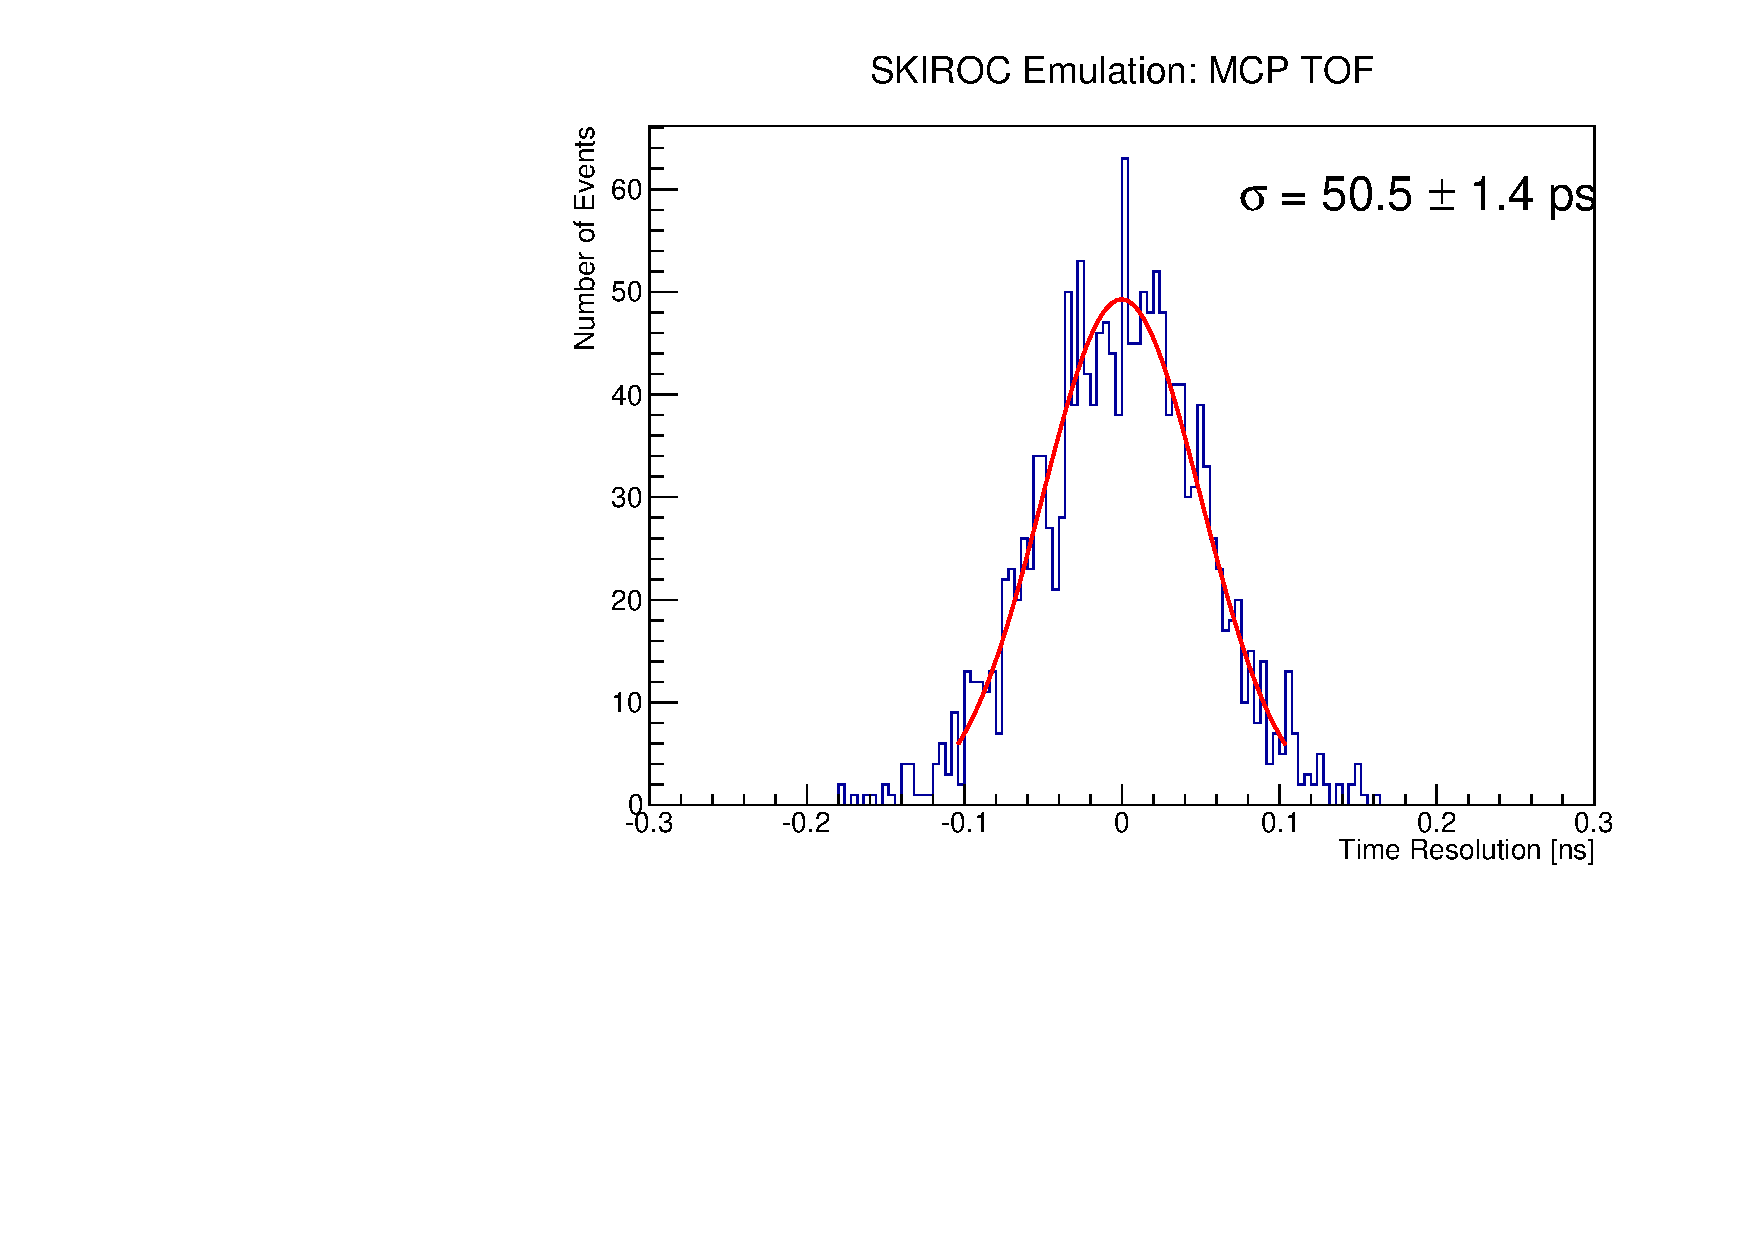
\includegraphics[width=\linewidth]{deltaTMCPSmear.pdf}
	\caption{Caption goes here}
	\label{peaks1}
	\end{minipage}\hfill
	\begin{minipage}{.5\textwidth}
	\centering
	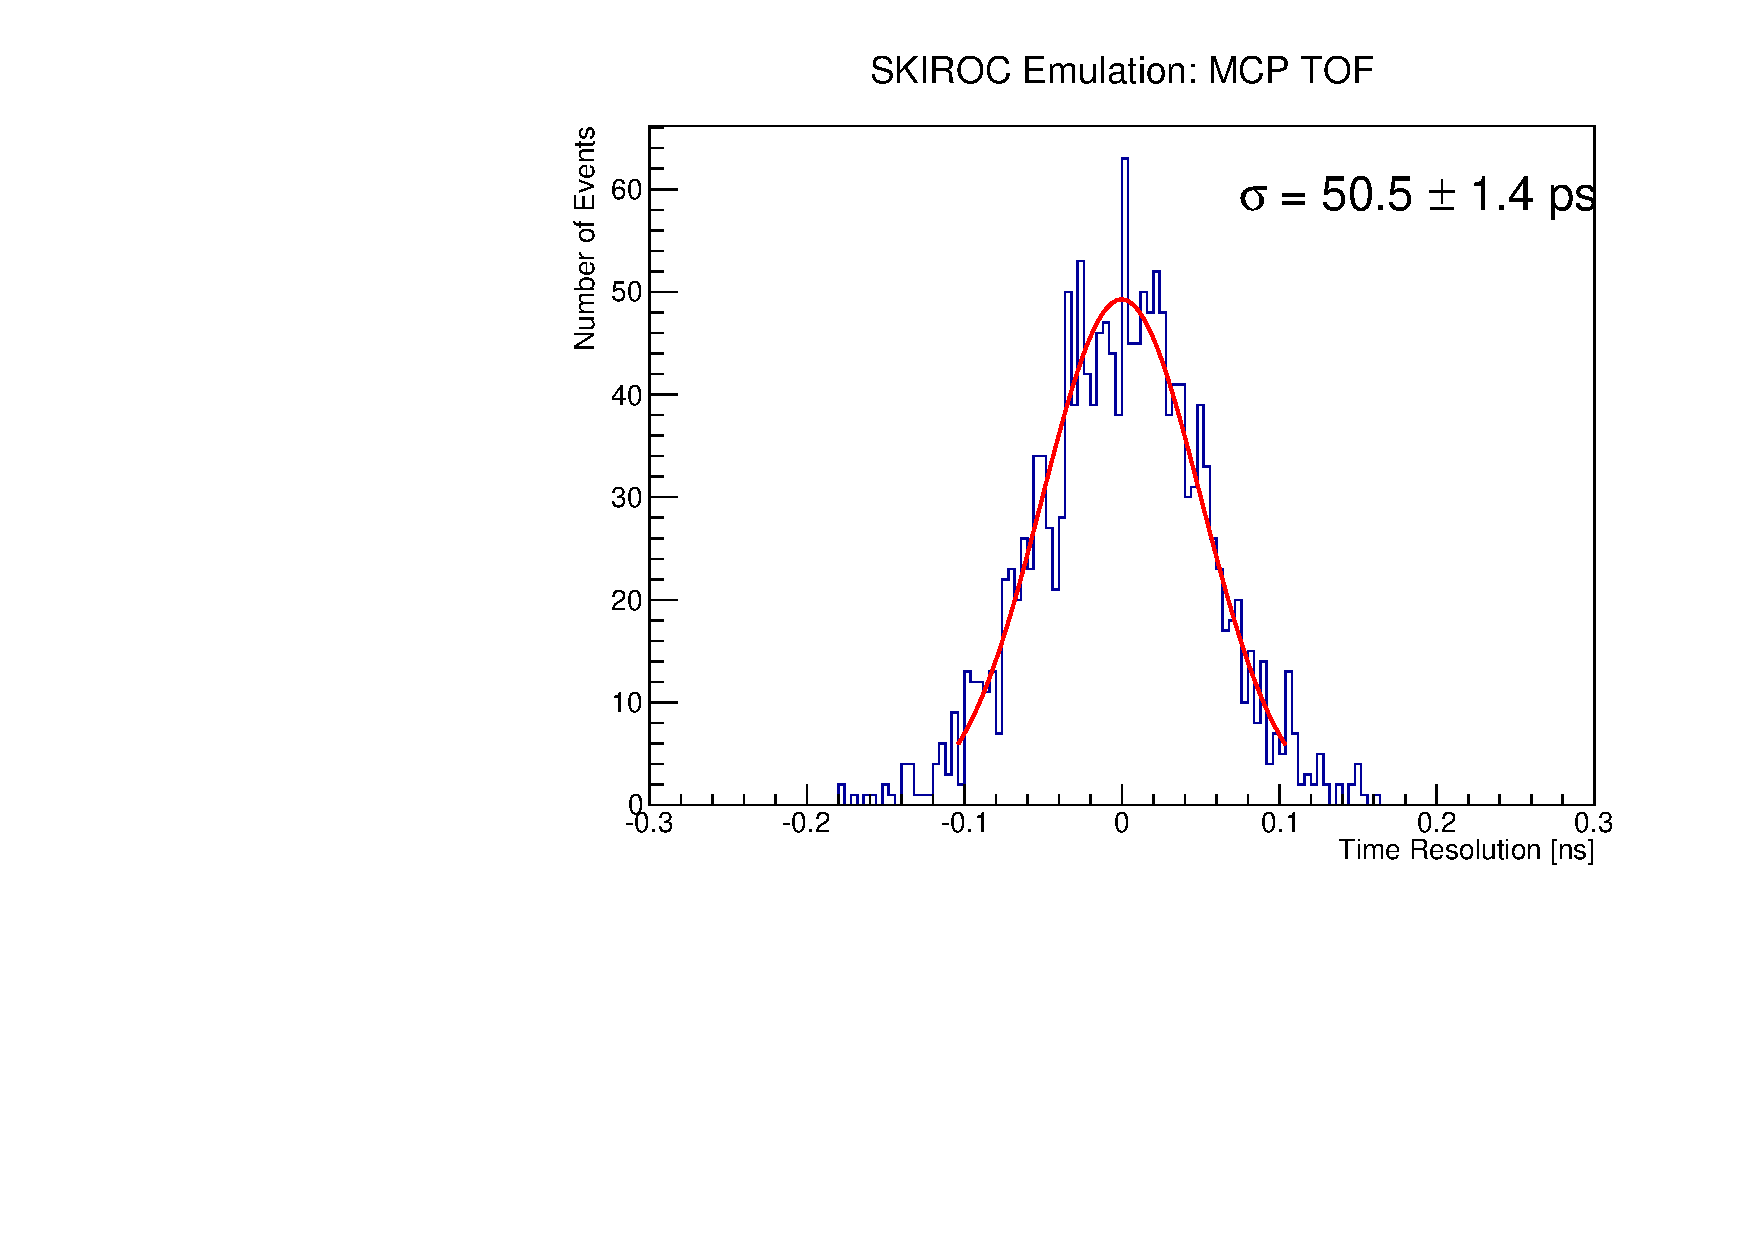
\includegraphics[width=\linewidth]{deltaTMCPSmear.pdf}
	\caption{Caption goes here}
	\label{peaks2}
	\end{minipage}
\end{figure}

look at \ref{peaks1} and \ref{peaks2}.
\end{comment}



\printbibliography

\end{document}
